\documentclass{article}

\usepackage{amsmath}
\usepackage{mdframed}
\usepackage{cases}
%\usepackage{subfigure}
\usepackage{subcaption}

\newcommand{\irow}[1]{% inline row vector
  \begin{smallmatrix}[#1]\end{smallmatrix}%
}

\usepackage{xfrac}
\usepackage{bbm}
\usepackage{multicol}
\usepackage{geometry}
\usepackage{multirow}
\usepackage{lscape}
\geometry{margin=1in}
\usepackage{hyperref}
\usepackage{color}



\providecommand{\e}[1]{\ensuremath{\times 10^{#1}}}

\title{Axisymmetric Nozzle Optimization Formulations\\DARPA EQUiPS SEQUOIA Team}
\author{Richard W. Fenrich\\Department of Aeronautics and Astronautics\\Stanford University, Stanford, CA\\rfenrich@stanford.edu}
\date{November 30, 2016}

\begin{document}

\maketitle

\tableofcontents

\listoftables

%\listoffigures

\section*{Nomenclature}

\begin{multicols}{2}
\begin{tabbing}
  XXX \= \kill% this line sets tab stop
  $A$ \> matrix of linear constraints \\
  $b$ \> linear constraint limits \\
  $c$ \> CDF probability level \\
  $F$ \> thrust \\
  $F_{req}$ \> required thrust \\
  KS \> Kreiselmeier-Steinhauser \\
  $g$ \> KS or PN or max function \\
  $l$ \> lower bounds on design variables \\
  $M$ \> mass \\
  $M_{req}$ \> maximum allowable mass \\
  $\hat{n}$ \> local normal coordinate \\
  PN \> modified P-norm \\ [\fill\columnbreak]
  $\hat{r}$ \> global radial coordinate \\
  $S$ \> stress failure criterion \\
  $T$ \> temperature \\
  $T_{max}$ \> max allowable temperature \\
  $u$ \> upper bounds on design variables \\
  $x$ \> deterministic variables \\
  $\hat{x}$ \> global axial coordinate \\
  $y$ \> design variables \\
  $\xi$ \> random parameters \\
  $\hat{\theta}$ \> global circumferential coordinate \\
  $\mu$ \> mean of quantity \\
  $\sigma$ \> stress failure criterion \\
  $\sigma_f$ \> stress criterion limit \\
 \end{tabbing}
\end{multicols}

\section{Introduction}

The purpose of this document is to unify the SEQUOIA team in pursuit of the same set of optimization problems. Section \ref{sec:models} describes the models used in the solution of the optimization problems and their common inputs and outputs. Section \ref{sec:generalOptimizationFormulations} describes the general robust, reliable, and aggressive optimization problem formulations.  Section \ref{sec:specificOptimizationFormulations} describes the associated specific formulations and equivalent deterministic formulation. Finally section \ref{sec:results} gives baseline results for the specific equivalent deterministic optimization problems considered in section \ref{sec:specificOptimizationFormulations}.

\section{Models} \label{sec:models}

The \texttt{MULTI-F} software brings together several design and analysis software codes of varying fidelities to provide comprehensive design and analysis capabilities for a military turbofan non-afterburning nozzle. Currently, only an axisymmetric nozzle is supported. \texttt{MULTI-F} models internal fluid flow, heat transfer through the nozzle wall, and temperature and total stress in the nozzle and its structure. The code can be accessed on GitHub at \url{<https://github.com/vmenier/MULTIF>}.

A common nozzle shape parameterization is used for each fidelity level. Figure \ref{fig:nozzleSchematic} shows the axisymmetric nozzle geometry and associated coordinate systems. Figure \ref{fig:components} shows the individual wall layers in the nozzle wall and a structural model of the nozzle with baffles and stringers.

\begin{mdframed}
\textbf{Components of the nozzle:} A nozzle component is defined as a part of the nozzle. These include the thermal layer, each layer in the load layer, each stringer, and each baffle. Since every stringer has the same shape, only one stringer needs to be considered as a component.
\end{mdframed}

\begin{figure}
\caption{Schematic of nozzle and geometric components showing global $\hat{x}$-$\hat{r}$ coordinate systems and one local $\hat{t}$-$\hat{n}$ coordinate system for the first wall layer, the thermal layer.}
\label{fig:nozzleSchematic}
\begin{center}
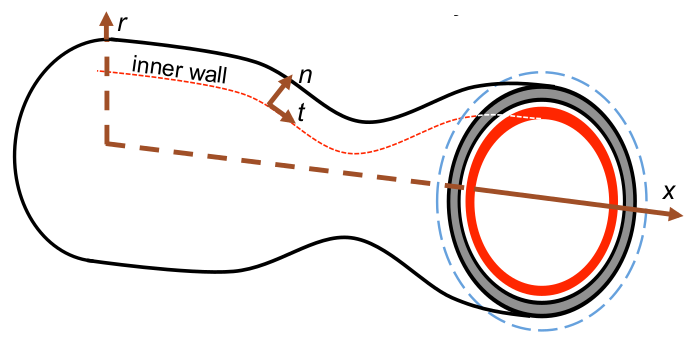
\includegraphics[scale=0.5]{figs/nozzle_schematic.png}
\end{center}
\end{figure}

\begin{figure}[t!]
    \centering
    \begin{subfigure}[t]{0.5\textwidth}
        \centering
        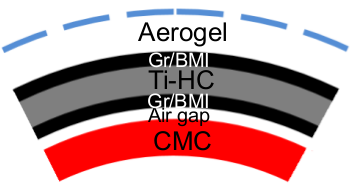
\includegraphics[width=0.9\linewidth]{figs/layers.png}
        \caption{Individual layers in the nozzle wall. The thermal insulation ``aerogel'' is not modeled but all other layers are modeled.}
    \end{subfigure}%
    ~ 
    \begin{subfigure}[t]{0.5\textwidth}
        \centering
        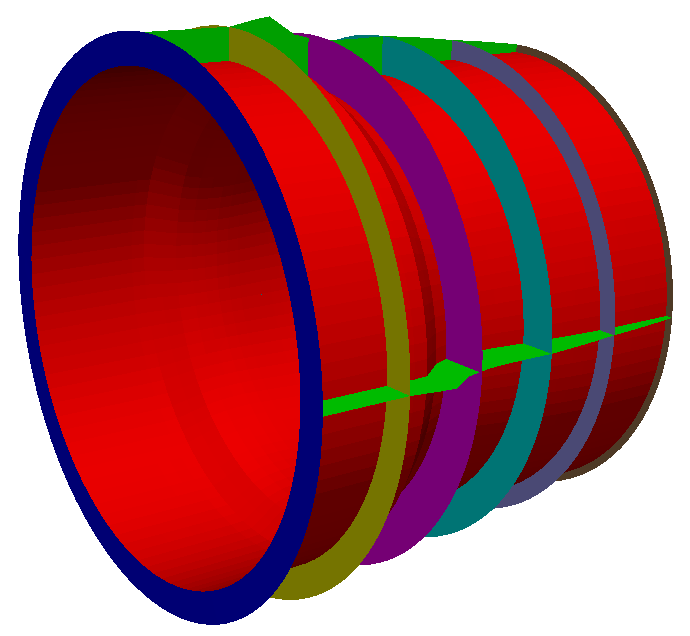
\includegraphics[width=0.6\linewidth]{figs/structural_model.png}
        \caption{Structural model of the nozzle showing nozzle wall, baffles, and stringers.}
    \end{subfigure}
    \caption{Nozzle components and structure.}
    \label{fig:components}
\end{figure}

\subsection{Inputs}

The inputs for the nozzle model are related to geometry, materials, inlet conditions, atmospheric conditions, and heat transfer to the ambient. Table \ref{tab:inputDimension} tallies the total dimension of the model inputs for various concrete parameterizations. A description of various inputs follows:

\begin{table}
\caption[Dimensions of model inputs]{Total dimension of model inputs for various parameterizations. The standard and high-dimension parameterization are the most realistic for real design problems.}
\label{tab:inputDimension}
\begin{center}
\begin{tabular}[]{ c | c | c | c}
\textbf{Input} & \textbf{Standard Param} & \textbf{High-Dim Param} & \textbf{Very High-Dim Param}\\ \hline
Inner wall geo            & 21  & 21   & 50   \\ \hline
Thermal layer geo         & 6   & 20   & 40   \\ \hline
Air layer geo             & 1   & 1    & 1    \\ \hline
Load layer geo            & 6*3 & 20*3 & 40*3 \\ \hline
Baffle geo                & 10  & 10   & 10   \\ \hline
Stringer geo              & 6   & 6    & 6    \\ \hline
CMC material              & 7   & 7    & 10   \\ \hline
GR-BMI material           & 20  & 20   & 20   \\ \hline
TI-HC material            & 7   & 7    & 9    \\ \hline
AIR material              & 1   & 1    & 1    \\ \hline
PANEL material            & 1   & 1    & 1    \\ \hline
Inlet conditions          & 2   & 2    & 4    \\ \hline
Atmospheric conditions    & 2   & 2    & 4    \\ \hline
Heat transfer coefficient & 1   & 2    & 4    \\ \hline \hline
\textbf{Total Dimension}  & 103 & 160  & 280  \\ \hline
\textbf{Total Deterministic Dimension} & \{0,62\} & \{0,118\} & \{0,227\} \\ \hline
\textbf{Total Random Dimension} & \{103,41\} & \{160,42\} & \{280,53\} \\ \hline
\end{tabular}
\end{center}
\end{table}

\begin{description}
\item[Analysis type] At the minimum, a fluid analysis must be performed, however thermal and structural analyses are optional.

\item[Inner wall geometry] The inner wall of the nozzle is parameterized using a 3rd degree basis spline (B-spline). The shape of the B-spline is manipulated by specifying a matrix of B-spline coefficients (\textit{i.e.} spline control points). The first two and last 2 coefficients must be the same. In addition, several degrees of freedom should be removed from control points near the throat to ensure only one degree of freedom controls the throat radius (see figure \ref{fig:throatDofs} in the Appendix (\ref{sec:appendix})). B-splines are also discussed in more detail in the Appendix (\ref{sec:appendix}).

\item[Thermal layer geometry] The thickness of the innermost wall layer is parameterized using a piecewise-linear function defined in the local non-orthogonal $\hat{x}$-$\hat{n}$ coordinate system, where $\hat{n}$ is the outward unit vector normal to the inner wall's B-spline. The function shape is controlled by manipulating the location of its breaks, and the function value at its breaks. A ceramic matrix composite material (CMC) is assigned to this layer.

\item[Air layer geometry] A constant thickness air layer is assumed to be present between the thermal and the load layers. This air layer has a physical thickness and is assumed to have isotropic properties used to estimate an equivalent thermal resistance between the thermal and load layers.

\item[Load layer geometry] The load layer is comprised of 3 individual layers, each with a thickness modeled separately using piecewise-linear functions defined in the local non-orthogonal $\hat{x}$-$\hat{n}$ coordinate systems, where $\hat{n}$ is the outward unit vector normal to the outside of the inner neighboring layer. Each layer's thickness distribution shape is controlled by manipulating the location of its breaks, and the function value at its breaks.The inner- and outermost layers use a composite material called Graphite-Bismaleimide (GR-BMI). The middle layer uses titanium honeycomb (TI-HC).

\item[Baffle geometry] Baffles (vertical panels perpendicular to the global $\hat{x}$-coordinate which provide structural support) are defined individually by the location of their centerline on $\hat{x}$, their thickness, and the distance they extend in the radial direction from the nozzle axis (height). Baffles are constructed from a symmetric 3-layer composite sandwich material (GR-BMI / TI-HC / GR-BMI), where the ratio of each layer thickness to baffle thickness is taken to be constant (and must be specified). The number of baffles is fixed for a given optimization problem, and is taken to be 6 in general. In addition, baffle height is by default automatically resized by \texttt{MULTI-F} to match the exterior wall profile.

\item[Stringer geometry] Stringers (long, thin structural elements which run the entire length of the outside of the nozzle) are spaced evenly about the circumference of the nozzle. Each stringer assumes the same geometry. The height ($\hat{r}$-direction length) and thickness ($\hat{\theta}$-direction length) are modeled using piecewise-linear functions, which share the same break locations, but can have different values at the breaks. Stringer break locations and heights can be automatically resized by \texttt{MULTI-F} to match baffle locations and heights.

\item[CMC material] The ceramic matrix composite (CMC) material is an isotropic material used by the thermal layer. It assumes no structural loads. Only density and thermal conductivity are needed inputs.

\item[GR-BMI material] The composite Graphite-Bismaleimide (GR-BMI) material is an anisotropic material used in the load layer, baffles, and stringers. Density, elastic moduli, shear modulus, Poisson ratio, mutual influence coefficients, thermal conductivities, and thermal expansion coefficients are needed inputs.

\item[TI-HC material] The titanium honeycomb (TI-HC) material is an anisotropic material used by the load layer and baffles, but is assumed to be isotropic. Density, elastic modulus, Poisson ratio, thermal conductivity, and thermal expansion coefficient are needed inputs.

\item[Inlet conditions] Nozzle inlet stagnation pressure and stagnation temperature must be specified. These are a function of flight conditions and engine conditions. Preset values can be used by specifying a mission.

\item[Atmospheric conditions] Atmospheric pressure and temperature must be specified. Preset values can be used by specifying a mission.

\item[Heat transfer coefficient to environment] This coefficient depends on flight conditions and atmospheric conditions and represents how well heat is transferred from the nozzle structure to the ambient environment.

\item[Fidelity-specific inputs] For low-fidelity this includes the error tolerance controlling the percent error in the conjugate heat transfer problem. For medium-fidelity this includes the mesh size (coarse, medium, or fine). In addition, fidelity of the thermostructural analysis is specified using a float ranging from 0 (low) to 1 (high).

\end{description}

\subsection{Outputs}

The outputs for each model include mass, volume, thrust, and various measures of stress failure criteria and temperature in almost every component. Stresses are calculated for each layer in the load layer and each baffle. Only thermal stresses are calculated for the thermal layer since pressure will equalize on both sides of the thermal layer. Temperatures are calculated in the thermal layer and each layer in the load layer but not for the baffles. A list of various outputs follows:

\begin{enumerate}
\item mass
\item volume
\item thrust
\item max failure stress criteria (for each component)
\item Kreiselmeier-Steinhauser (KS) of failure stress criteria (for each component)
\item modified P-norm (PN) of failure stress criteria (for each component)
\item max temperature (for each component)
\item Kreiselmeier-Steinhauser (KS) of temperature field (for each component)
\item modified P-norm (PN) of temperature field (for each component)
\end{enumerate}

\textit{Note 1:} The mass and volume calculation for the nozzle includes the nozzle wall, stringers, and baffles and is calculated via numerical integration of each layer in the nozzle wall.

\textit{Note 2:} The failure stress criteria consists of an appropriate failure criterion associated with each FEM-nodal stress for each component. For TI-HC this is the von Mises failure criterion; for GR-BMI and CMC, this is a variation of the maximum strain failure criterion.

\textit{Note 3:} Kreiselmeier-Steinhauser (KS) and modified P-norm (PN) functions are common methods for replacing a large number of constraints (\textit{i.e.} a local stress or temperature constraint on every FEM node) with a single constraint. The Appendix (\ref{sec:appendix}) provides more information on these functions.

\subsection{Fidelity Levels}

\subsubsection{Low-Fidelity}

The low-fidelity model solves a conjugate heat transfer problem to calculate nozzle flow and wall temperatures. The nozzle internal flow is estimated using a quasi-1D area-averaged Navier-Stokes ordinary differential equation and heat transfer is estimated using linear resistances for each nozzle component. Heat is only allowed to flow in each layer's local normal coordinate $\hat{n}$. Stresses are calculated using AERO-S. If a thermal analysis is enabled, then AERO-S will run its own thermal analysis but uses the inner wall temperature provided by the low-fidelity aero model.

\subsubsection{Medium-Fidelity}

The medium-fidelity model currently assumes an adiabatic inner wall and solves for the nozzle flow using SU2's Euler implementation. A local relaxation number is used to robustly achieve convergence over a wide range of geometries. Then AERO-S is used to calculate heat transfer through the wall and stresses. 

\subsubsection{High-Fidelity}

The high-fidelity model is still being implemented. It will use a Reynolds-averaged Navier-Stokes implementation. In addition, the nozzle geometry will not be axisymmetric. AERO-S will still be used to calculate heat transfer and stresses, with the additional option of using a non-linear calculation.

\subsubsection{Other Fidelities}

In addition, other high(er) fidelity levels are under consideration.

\section{General Optimization Formulations} \label{sec:generalOptimizationFormulations}

Three design approaches were addressed in the proposal: robust design, reliable design, and aggressive design. The optimization formulations make reference to nozzle components and properties via their associated index which can be found in Table \ref{tab:componentIndexing}. 

\begin{mdframed}
\textbf{Notation for optimization formulations:}  
\begin{description}
\item[Variables] Design variables (deterministic or random) are contained in the vector $y$. Other random parameters (not design variables) are contained in the vector $\xi$. Function dependencies on fixed deterministic variables $x$ are dropped; however deterministic variables $x_i \in \{y_i\}$ if $x_i$ is a design variable. Lastly, $\mu_y = E[y]$ and $\mu_{\xi} = E[\xi]$.

\item[Quantities of interest] The following quantities of interest are specified: mass $M(y)$, thrust $F(y,\xi)$, temperature field for component $i$ $T_i(y,\xi)$, and stress failure criterion for component $i$ $S_i (\sigma_i(y,\xi) )$ which is a function of the stresses $\sigma_i$ in component $i$. Constraint agglomeration functions such as KS or modified P-norm functions (\ref{sec:appendix}) are notated by $g_j(\ldots)$. 

\item[Constraint limits] $M_{req}$ denotes the maximum allowable mass, $F_{req}$ denotes the required amount of thrust, $T_{max,i}$ denotes the maximum allowable temperature for component $i$. $Ay \leq b$ is a set of required linear constraints and $l$ and $u$ are lower and upper bounds on the design variables $y$.
\end{description}
\end{mdframed}

\begin{table}
\caption[Component indexing matrix]{Component indexing matrix.}
\label{tab:componentIndexing}
\begin{center}
\begin{tabular}[]{ c | c | c | c | c }
\textbf{Component} & \textbf{Index} & \textbf{Material} & \textbf{$T_{max,i}$} (K) & \textbf{Failure criteria} \\ \hline
Thermal layer & 1 & CMC & 973 & max principle failure strain \\ \hline
(Air layer) & N/A & air & N/A & N/A \\ \hline
Load layer (inner) & 2 & GR-BMI & 505.15 & max local failure strain \\ \hline
Load layer (middle) & 3 & TI-HC & 755 & von Mises \\ \hline
Load layer (outer) & 4 & GR-BMI & 505.15 & max local failure strain \\ \hline
Stringer & 5 & GR-BMI & N/A & max local failure strain \\ \hline
Baffle 1 (left-most) & 6 & GR-BMI/TI-HC & N/A & von Mises \\ \hline
$\ldots$ & $\ldots$ & $\ldots$ & $\ldots$ & $\ldots$ \\ \hline
Baffle 6 (right-most) & 11 & GR-BMI/TI-HC & N/A & von Mises \\ \hline
\end{tabular}
\end{center}
\end{table}

\pagebreak
\subsection{Robust Design}

The robust design formulation aims to obtain robust thrust while meeting necessary mass, thrust, temperature, and stress expectation constraints. Note that the equivalent deterministic formulation is a feasibility problem with many possible solutions.

\begin{multicols}{2}
\centering
Reliable formulation:
\begin{equation}
\label{eq:general_robust_optim}
\begin{aligned}
& \underset{y}{\text{minimize}}
% objective function:
& & \textrm{Var} \left( F(y,\xi) \right) \\
& \text{subject to}
% constraints:
& & E \left[ M(y) \right] \leq M_{req} \\
& & & E \left[ F(y,\xi) \right] \geq F_{req} \\
& & & E \left[ g_1 \left( T_1(y,\xi) \right) \right] \leq T_{max,1} \\
& & & \vdots \\
& & & E \left[ g_4 \left( T_4(y,\xi) \right) \right] \leq T_{max,4} \\
& & & E \left[ g_5 \left( S_1 ( \sigma_1(y,\xi) ) \right) \right] \leq 1 \\
& & & \vdots \\
& & & E \left[ g_{15} \left( S_{11} ( \sigma_{11}(y,\xi)  ) \right) \right] \leq 1 \\
& & & Ay \leq b \\
& & & l \leq y \leq u \\
\end{aligned}
\end{equation}
\vfill \columnbreak
Deterministic formulation: 
\begin{equation}
\label{eq:general_robust_equiv_deterministic_optim}
\begin{aligned}
& \underset{\mu_y}{\text{minimize}}
% objective function:
& & 0^T\mu_y \\
& \text{subject to}
% constraints:
& & M(\mu_y) \leq M_{req} \\
& & & F(\mu_y,\mu_{\xi}) \geq F_{req} \\
& & & g_1 \left( T_1(\mu_y,\mu_{\xi}) \right) \leq T_{max,1} \\
& & & \vdots \\
& & & g_4 \left( T_4(\mu_y,\mu_{\xi}) \right) \leq T_{max,4} \\
& & & g_5 \left( S_1 ( \sigma_1(\mu_y,\mu_{\xi}) ) \right) \leq 1 \\
& & & \vdots \\
& & & g_{15} \left( S_{11} ( \sigma_{11}(\mu_y,\mu_{\xi}) ) \right) \leq 1 \\
& & & A\mu_y \leq b \\
& & & l \leq \mu_y \leq u \\
\end{aligned}
\end{equation}
\end{multicols}

\subsection{Reliable Design}

The reliable design formulation aims to obtain a lightweight nozzle while obtaining reliable thrust, and temperature and stress performance.

\begin{multicols}{2}
\centering
Reliable formulation:
\begin{equation}
\label{eq:general_reliable_optim}
\begin{aligned}
& \underset{y}{\text{minimize}}
% objective function:
& & E[M(y)] \\
& \text{subject to}
% constraints:
& & P \left[ F(y,\xi) \leq F_{req} \right] \leq c_1 \\
& & & P \left[ g_1 \left( T_1(y,\xi) \right) > T_{max,1} \right] \leq c_{2} \\
& & & \vdots \\
& & & P \left[ g_4 \left( T_4(y,\xi) \right) > T_{max,4} \right] \leq c_{5} \\
& & & P \left[ g_5 \left( S_1 ( \sigma_1(y,\xi) ) \right) > 1 \right] \leq c_{6} \\
& & & \vdots \\
& & & P \left[ g_{15} \left( S_{11} ( \sigma_{11}(y,\xi) ) \right) > 1 \right] \leq c_{15} \\
& & & Ay \leq b \\
& & & l \leq y \leq u \\
\end{aligned}
\end{equation}
\vfill \columnbreak
Deterministic formulation: 
\begin{equation}
\label{eq:general_reliable_equiv_deterministic_optim}
\begin{aligned}
& \underset{\mu_y}{\text{minimize}}
% objective function:
& & M(\mu_y) \\
& \text{subject to}
% constraints:
& & F(\mu_y,\mu_{\xi}) \geq F_{req} \\
& & & g_1 \left( T_1(\mu_y,\mu_{\xi}) \right) \leq T_{max,1} \\
& & & \vdots \\
& & & g_4 \left( T_4(\mu_y,\mu_{\xi}) \right) \leq T_{max,4} \\
& & & g_5 \left( S_1 ( \sigma_1(\mu_y,\mu_{\xi}) ) \right) \leq 1 \\
& & & \vdots \\
& & & g_{15} \left( S_{11} ( \sigma_{11}(\mu_y,\mu_{\xi}) ) \right) \leq 1 \\
& & & A\mu_y \leq b \\
& & & l \leq \mu_y \leq u \\
\end{aligned}
\end{equation}
\end{multicols}

\subsection{Aggressive Design}

Aggressive design attempts to find a design with quantity of interest PDFs that match designer-specified PDFs as closely as possible. To date, no aggressive design formulation has been specified.

\subsection{Shared Aspects}

\subsubsection{Design Variables $y$}

Since all problems are a shape design problem the design variables $y$ are related to the geometry of the nozzle. The following parameters can be considered design variables (deterministic or random):

\begin{enumerate}
\item A subset of the coordinates of the inner wall B-spline's coefficients.
\item The location and value of breaks in any wall layer geometry parameterization.
\item The constant thickness of the air gap between the thermal and load layers.
\item The location and thickness of baffles.
\item The location of breaks, and values of height and thickness at the breaks for a stringer.
\end{enumerate}

The geometry above could be considered random due to manufacturing tolerances.

\subsubsection{Random Parameters $\xi$}

Random parameters are inputs to quantities of interest, but not design variables. They include:

\begin{enumerate}
\item Material properties for each material.
\item Inlet conditions.
\item Atmospheric conditions.
\item Heat transfer coefficient to the environment.
\end{enumerate}

\subsubsection{Linear Constraints $Ay \leq b$}

The set of linear constraints $Ay \leq b$ is used to avoid numerical issues and impossible geometries during the course of the optimization. \textit{It should be implemented for every optimization.} The size of the matrix $A$ will depend on the design variables. The list below describes what linear constraints should be used for certain design variables.

\begin{description}
\item[B-spline coefficients $c_i \in y$:] $A$ should include: 1) The $\hat{x}$-coordinates of neighboring control points should not crossover each other, 2) the pre-throat geometry should monotonically converge, 3) the control points governing the nozzle throat should remain below all other control points, 4) the absolute value of the slope of the line drawn between two adjacent control points should be less than a certain value, and 5) slopes drawn between adjacent control points next to the throat should not be too large. The fourth constraint is a surrogate for limiting the slope of the B-spline itself, but proves useful due to the fact that sections of the B-spline lie within a convex hull of neighboring coefficients. The fifth constraint is a surrogate for managing a gradual slope change at the throat of the nozzle.
\item[Location and value of breaks for any wall layer $\in y$:] $A$ should include: 1) Break locations should be separated by at least a given distance, and 2) The absolute value of the slope of the line drawn between two adjacent breaks should be less than a certain value.
\item[Location and thickness of baffles $\in y$:] $A$ should include: 1) Baffles should be separated by at least a given distance, and 2) Adjacent baffles should be within at least a given distance.
\item[Location of breaks, and height and thickness at breaks for stringer $\in y$:] $A$ should include the same constraints at those for the wall layers.
\end{description}

\section{Specific Optimization Formulations} \label{sec:specificOptimizationFormulations}

\subsection{Material Constants}

Material properties are specified using the local coordinate system in figure \ref{fig:materialCoordinateSystem}. An incomplete set of material properties is gathered from a variety of experimental data sources. Missing macroscopic properties are either determined through fundamental physical analysis of the material's structure or are approximated by values for similar materials. Table \ref{tab:matPropCMC} provides the properties used in the \texttt{MULTI-F} analysis for the CMC material, table \ref{tab:matPropGR-BMI} for the GR-BMI material, table \ref{tab:matPropTI-HC} for the TI-HC material, and table \ref{tab:matPropAirGap} for the air gap.

\begin{figure}
\caption{Local coordinate system used for the specification of material properties in shell materials.}
\label{fig:materialCoordinateSystem}
\begin{center}
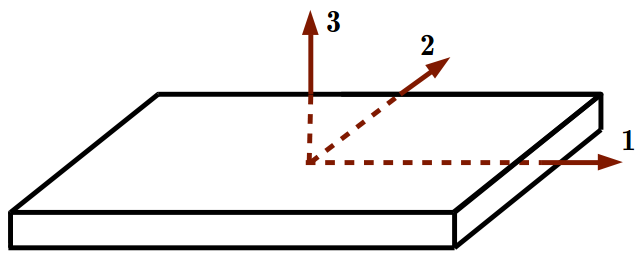
\includegraphics[scale=0.3]{figs/material_directions.png}
\end{center}
\end{figure}

\begin{table}
\caption[CMC material properties]{Assumed \textit{isotropic} material properties for the heat layer's ceramic matrix composite material (CMC).}
\label{tab:matPropCMC}
\begin{center}
\begin{tabular}[]{ c | c | c | c | c }
\textbf{Property} & \textbf{symbol} & \textbf{Units} & \textbf{Nominal Value} & \textbf{Distribution} \\ \hline
Density & $\rho$ & $\frac{\textrm{kg}}{\textrm{m}^3}$ & 2410 & $\textrm{ln}\mathcal{N}(7.7803,0.0182^2)$ \\ \hline
Elastic modulus & $E$ & GPa & 67.1 & $\textrm{ln}\mathcal{N}(4.2047,0.0551^2)$ \\ \hline
%$G_{12}$ & GPa & unknown & \\ \hline
Poisson ratio & $\nu$ & & 0.33 & $\mathcal{U}(0.23,0.43)$\\ \hline
Thermal conductivity & $k$ & $\frac{\textrm{W}}{\textrm{m-K}}$ & 1.41 & $\mathcal{U}(1.37,1.45)$ \\ \hline
Thermal expansion coefficient & $\alpha$ & $\textrm{K}^{-1} \times 10^{-6}$ & 0.24 & $\mathcal{U}(0.228,0.252)$ \\ \hline \hline
Max service temperature & $T_{max}$ & K & 973 & $\mathcal{U}(963,983)$ \\ \hline
Failure strain* & $\epsilon_{f}$ & \% & 0.07 & $\textrm{ln}\mathcal{N}(-2.6694,0.1421^2)$ \\ \hline
\end{tabular} \\
*if failure by yield (von Mises) is assumed instead of failure by strain (for simplicity), use yield stress $\sigma_Y = 120$ MPa, where $\sigma_Y \sim \textrm{ln}\mathcal{N}(4.7803,0.1196)$.
\end{center}
\end{table}

\begin{table}
\caption[Gr-BMI material properties]{Macroscopic laminate material properties for the load layer's graphite/bismaleimide (GR-BMI) composite layers used in the axisymmetric shell specification.}
\label{tab:matPropGR-BMI}
\begin{center}
\begin{tabular}[]{ c | c | c | c | c }
\textbf{Property} & \textbf{Symbol} & \textbf{Units} & \textbf{Nominal Value} & \textbf{Distribution} \\ \hline
Density & $\rho$ & $\frac{\textrm{kg}}{\textrm{m}^3}$ & 1568 & $\mathcal{U}(1563,1573)$ \\ \hline
Elastic moduli & $E_{1} = E_{2}$ & GPa & 60 & $\mathcal{U}(57,63)$ \\ \hline
In-plane shear modulus & $G_{12}$ & GPa & 23.31 & $\mathcal{U}(22.6,24.0)$ \\ \hline
Poisson ratios & $\nu_{12} = \nu_{21}$ & & 0.344 & $\mathcal{U}(0.334,0.354)$\\ \hline
Mutual influence coef (first kind) & $\mu_{1,12} = \mu_{2,12}$ & & 0.0 & $\mathcal{U}(-0.1,0.1)$ \\ \hline
Mutual influence coef (second kind) & $\mu_{12,1} = \mu_{12,2}$ & & 0.0 & $\mathcal{U}(-0.1,0.1)$ \\ \hline
Thermal conductivity & $k_{1} = k_{2}$ & $\frac{\textrm{W}}{\textrm{m-K}}$ & 3.377 & $\mathcal{U}(3.208,3.546)$ \\ \hline
Thermal conductivity & $k_{3}$ & $\frac{\textrm{W}}{\textrm{m-K}}$ & 3.414 & $\mathcal{U}(3.243,3.585)$ \\ \hline
Thermal expansion coef & $\alpha_{1} = \alpha_{2}$ & $\textrm{K}^{-1} \times 10^{-6}$ & 1.200 & $\mathcal{U}(1.16,1.24)$ \\ \hline
Thermal expansion coef & $\alpha_{12}$ & $\textrm{K}^{-1} \times 10^{-6}$ & 0.0 & $\mathcal{U}(-0.04,0.04)$ \\ \hline \hline
Max service temperature & $T_{max}$ & K & 505 & $\mathcal{U}(500,510)$ \\ \hline
Failure strain (tension)* & $\epsilon_{f,1} = \epsilon_{f,2}$ & \% & 0.75 & $\mathcal{U}(0.675,0.825)$ \\ \hline
Failure strain (compression)* & $\epsilon_{f,1} = \epsilon_{f,2}$ & \% & -0.52 & $\mathcal{U}(-0.572,-0.494)$ \\ \hline
%Failure strain (tension/compression) & $\epsilon_{f,3}$ & \% & 0.17/0.11 \\ \hline
Failure strain (shear)* & $\gamma_{f}$ & \% & 0.17 & $\mathcal{U}(0.153,0.187)$ \\ \hline
\end{tabular} \\
*if failure by yield (von Mises) is assumed instead of failure by strain (for simplicity), use isotropic yield stress $\sigma_Y = 324$ MPa, where $\sigma_Y \sim \textrm{ln}\mathcal{N}(5.7736,0.1196)$.
\end{center}
\end{table}

\begin{table}
\caption[TI-HC material properties]{Assumed \textit{isotropic} macroscopic material properties for titanium honeycomb layer (TI-HC).}
\label{tab:matPropTI-HC}
\begin{center}
\begin{tabular}[]{ c | c | c | c | c }
\textbf{Property} & \textbf{Symbol} & \textbf{Units} & \textbf{Nominal Value} & \textbf{Distribution} \\ \hline
%Density & $\rho$ & $\frac{\textrm{kg}}{\textrm{m}^3}$ & 101.696 & $\mathcal{U}(\pm1\textrm{\%})$ \\ \hline
% Density, nominal +/- 1%, Bencor, Inc.
Density & $\rho$ & $\frac{\textrm{kg}}{\textrm{m}^3}$ & 179.57 & $\mathcal{U}(177.77,181.37)$ \\ \hline
% Elastic modulus: nominal, NASA report 101732
%Elastic modulus& $E$ & GPa & 0.1915 &  \\ \hline
% Elastic modulus: nominal, Bencor, Inc.
Elastic modulus& $E$ & GPa & 0.190 & $\textrm{ln}\mathcal{N}(0.6441,0.0779^2)$ \\ \hline
%$E_{3}$ & GPa & 1.915 & \\ \hline
%$G_{12}$ & GPa & $4.2 \times 10^{-8}$ & \\ \hline
%$G_{23}$ & GPa & 1.248 & \\ \hline
%$G_{31}$ & GPa & 0.565 & \\ \hline
% Poisson ratio: nominal, NASA report 101732
%Poisson ratio & $\nu$ & & 0.00658 & \\ \hline
% Poisson ratio: estimate using Bencor, Inc. E and G and isotropic relation
Poisson ratio & $\nu$ & & 0.178 & $\mathcal{U}(0.160,0.196)$ \\ \hline
% Thermal conductivity: Nominal, source: analytical estimate from Lewis-Nielson Semi-theoretical model using NASA report 101732 density
%Thermal conductivity & $k$ & $\frac{\textrm{W}}{\textrm{m-K}}$ & 0.413 &  $\mathcal{U}(0.403,0.421)$ \\ \hline
% Thermal conductivity: Nominal +/- 4%, source: analytical estimate from Lewis-Nielson Semi-theoretical model using Bencor, Inc. datasheet density
Thermal conductivity & $k$ & $\frac{\textrm{W}}{\textrm{m-K}}$ & 0.708 &  $\mathcal{U}(0.680,0.736)$ \\ \hline
% Thermal expansion coef: Nominal, source: NASA report 101732
Thermal expansion coefficient & $\alpha$ & $\textrm{K}^{-1} \times 10^{-6}$ & 2.97 & $\mathcal{U}(2.88,3.06)$ \\ \hline \hline
% Max service temperature: Nominal, source: online
Max service temperature & $T_{max}$ & K & 755 &  $\mathcal{U}(745,765)$ \\ \hline
% Yield stress: Nominal, source: NASA report 101732
%Yield stress & $\sigma_Y$ & MPa & 8.04 & \\ \hline
% Yield stress: Nominal +/- 2 exp. standard deviations of 1.56, source: Bencor, Inc. datasheet
Yield stress & $\sigma_Y$ & MPa & 12.9 & $\textrm{ln}\mathcal{N}(2.5500,0.1205^2)$ \\ \hline
\end{tabular}
\end{center}
\end{table}

\begin{table}
\caption[Air gap material properties]{Assumed properties of air gap between thermal and load layers.}
\label{tab:matPropAirGap}
\begin{center}
\begin{tabular}[]{ c | c | c | c | c }
\textbf{Property} & \textbf{Symbol} & \textbf{Units} & \textbf{Nominal Value} & \textbf{Distribution} \\ \hline
Density & $\rho$ & $\frac{\textrm{kg}}{\textrm{m}^3}$ & 0 & N/A \\ \hline
% Based on values from Engineeringtoolbox.com
Thermal conductivity & $k$ & $\frac{\textrm{W}}{\textrm{m-K}}$ & 0.0425 &  $\mathcal{U}(0.0320,0.0530)$ \\ \hline
\end{tabular}
\end{center}
\end{table}

\subsection{Mission Parameters}

A typical reconnaissance mission was analyzed for a small high-subsonic unmanned military aircraft. The mission includes climbing as fast as possible to a cruise altitude of 43,000 ft, cruising at Mach 0.92 for a specified distance to an observation point, say 500 km, loitering at an altitude of 43,000 ft and Mach 0.5 for 2 hours and then returning to the takeoff point. On the return, the aircraft descends to 10,000 ft and cruises at Mach 0.9 in a high-speed ``dash'' segment lasting several kilometers before landing (see figure \ref{fig:missionSchematic}). The analysis of this mission showed that the climb segment was the most critical for nozzle performance since maximum thrust was required at all altitudes leading to the highest temperatures and pressures at the inlet of the nozzle. In particular, the state of climb right before beginning the cruise segment was the most critical in terms of stresses and temperatures experienced by the nozzle. Table \ref{tab:missionParams} summarizes the mission parameters used in the nozzle analysis.

\begin{table}
\caption[Mission parameters]{Mission parameters.}
\label{tab:missionParams}
\begin{center}
\begin{tabular}[]{ c | c | c | c }
\textbf{Parameter} & \textbf{Units} & \textbf{Nominal Value} & \textbf{Distribution} \\ \hline
Altitude & ft (km) & 40,000 (12.192) & N/A \\ \hline
Mach & & 0.511 & N/A \\ \hline
Required Thrust & N & 21,500 & N/A \\ \hline
Inlet stagnation pressure & Pa & 97,585 & $\textrm{ln}\mathcal{N}(11.5010, 0.0579^2)$ \\ \hline
Inlet stagnation temperature & K & 955.0 & $\textrm{ln}\mathcal{N}(6.8615, 0.0119^2)$ \\ \hline
% Atmospheric distributions taken from assumed log normal data for January at 60degN
% Atmospheric pressure Gaussian distribution is $\mathcal{N}(18754,606^2))$
Atmospheric pressure & Pa & 18,754 & $\textrm{ln}\mathcal{N}(9.8386,0.0323^2)$ \\ \hline
% Atmospheric temperature Gaussian distribution is $\mathcal{N}(216.7,6.11^2)$
Atmospheric temperature & K & 216.7 & $\textrm{ln}\mathcal{N}(5.3781,0.0282^2)$ \\ \hline
Heat transfer coefficient to environment & $\frac{\textrm{W}}{\textrm{m}^2\textrm{-K}}$ & 12.62 & $\textrm{ln}\mathcal{N}(2.5090,0.2285)$ \\ \hline
\end{tabular}
\end{center}
\end{table}

\begin{figure}
\caption{Schematic of typical reconnaissance mission with critical top-of-climb segment circled.}
\label{fig:missionSchematic}
\begin{center}
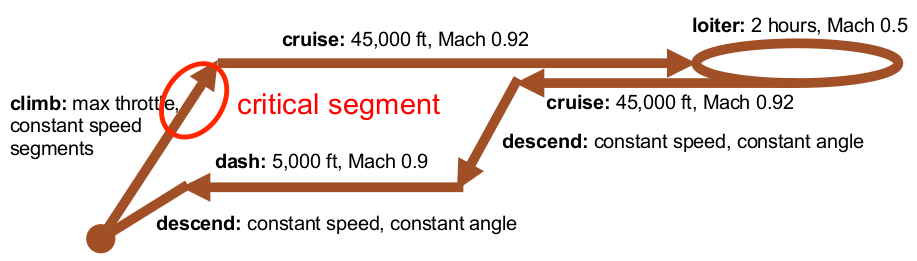
\includegraphics[scale=0.4]{figs/mission_profile.png}
\end{center}
\end{figure}

\subsection{Geometric Parameters}

Table \ref{tab:geoParams} records the reasonable ranges (bounds) and nominal values of all necessary geometric parameters.

\begin{table}
\caption[Bounds for design variables]{Bounds for nozzle design variables}
\label{tab:geoParams}
\begin{center}
\begin{tabular}[]{ c | c | c | c | c}
\textbf{Parameter} & \textbf{Units} & \textbf{Nominal Value} & \textbf{Lower Bound} & \textbf{Upper Bound} \\ \hline
Wall B-spline coefs & m & varies & min(-10\%,0) & +10\% \\ \hline
All layer thickness locations (non-dim) & & varies & 0 & 1 \\ \hline
Thermal layer thickness & m & 0.03 & 0.01 & 0.05 \\ \hline
Air gap thickness & m & 0.005 & 0.003 & 0.01 \\ \hline
Inside load layer thickness & m & 0.002 & 0.0005 & 0.01 \\ \hline
Middle load layer thickness & m & 0.013 & 0.0064 & 0.0159 \\ \hline
Outside load layer thickness & m & 0.002 & 0.0005 & 0.01 \\ \hline
Number of stringers & & 4 & 2 & 12+ \\ \hline
Stringer thickness locations (non-dim) & & varies & 0 & 1 \\ \hline
Stringer thickness & m & 0.01 & 0.002 & 0.01 \\ \hline
Stringer height & m & N/A & N/A & N/A \\ \hline
Number of baffles & & 6 & 2 & 6+ \\ \hline
Baffle location (non-dim) &  & varies & 0 & 1 \\ \hline
Baffle thickness & m & 0.01 & 0.0074 & 0.0359 \\ \hline
Baffle height & m & N/A & N/A & N/A \\ \hline
\end{tabular}
\end{center}
\end{table}

\subsection{Robust Design}

\subsubsection{Full Problem Formulation}

\begin{mdframed}
\textbf{Choice of Mass Constraint:}  
Total mass of the baseline (nominal) nozzle and surrounding structure is 118.74968232... kg. A 20\% weight reduction is considered excellent, although the reduction can perhaps be greater. Thus $M_{req}$ is taken to be 95 kg.
\end{mdframed}

\begin{multicols}{2}
\centering
Reliable formulation:
\begin{equation}
\label{eq:specific_robust_optim}
\begin{aligned}
& \underset{y}{\text{minimize}}
% objective function:
& & \textrm{Var} \left( F(y,\xi) \right) \\
& \text{subject to}
% constraints:
& & E \left[ M(y) \right] \leq 95 \\
& & & E \left[ F(y,\xi) \right] \geq 21500 \\
& & & E \left[ g_1 \left( \sfrac{T_2(y,\xi)}{T_{max,2}} \right) \right] \leq 1 \\
& & & E \left[ g_2 \left( S_1 ( \sigma_1(y,\xi) ) \right) \right] \leq 1 \\
& & & E \left[ g_3 \left( S_2 ( \sigma_2(y,\xi) ) \right) \right] \leq 1 \\
& & & E \left[ g_4 \left( S_3 ( \sigma_3(y,\xi) ) \right) \right] \leq 1 \\
& & & E \left[ g_5 \left( S_4 ( \sigma_4(y,\xi) ) \right) \right] \leq 1 \\
& & & E \left[ g_6 \left( S_5 ( \sigma_5(y,\xi) ) \right) \right] \leq 1 \\
& & & E \left[ g_7 \left( S_6 ( \sigma_6(y,\xi) ) \right) \right] \leq 1 \\
& & & E \left[ g_8 \left( S_7 ( \sigma_7(y,\xi) ) \right) \right] \leq 1 \\
& & & E \left[ g_9 \left( S_8 ( \sigma_8(y,\xi) ) \right) \right] \leq 1 \\
& & & E \left[ g_{10} \left( S_9 ( \sigma_9(y,\xi) ) \right) \right] \leq 1 \\
& & & E \left[ g_{11} \left( S_{10} ( \sigma_{10}(y,\xi) ) \right) \right] \leq 1 \\
& & & E \left[ g_{12} \left( S_{11} ( \sigma_{11}(y,\xi)  ) \right) \right] \leq 1 \\
& & & Ay \leq b \\
& & & l \leq y \leq u \\
\end{aligned}
\end{equation}
\vfill \columnbreak
Deterministic formulation: 
\begin{equation}
\label{eq:specific_robust_equiv_deterministic_optim}
\begin{aligned}
& \underset{\mu_y}{\text{minimize}}
% objective function:
& & 0^T\mu_y \\
& \text{subject to}
% constraints:
& & M(\mu_y) \leq 95 \\
& & & F(\mu_y,\mu_{\xi}) \geq 21500 \\
& & & g_1 \left( \sfrac{T_1(\mu_y,\mu_{\xi})}{T_{max,2}} \right) \leq 1 \\
& & & g_2 \left( S_1 ( \sigma_1(\mu_y,\mu_{\xi}) ) \right) \leq 1 \\
& & & g_3 \left( S_2 ( \sigma_2(\mu_y,\mu_{\xi}) ) \right) \leq 1 \\
& & & g_4 \left( S_3 ( \sigma_3(\mu_y,\mu_{\xi}) ) \right) \leq 1 \\
& & & g_5 \left( S_4 ( \sigma_4(\mu_y,\mu_{\xi}) ) \right) \leq 1 \\
& & & g_6 \left( S_5 ( \sigma_5(\mu_y,\mu_{\xi}) ) \right) \leq 1 \\
& & & g_7 \left( S_6 ( \sigma_6(\mu_y,\mu_{\xi}) ) \right) \leq 1 \\
& & & g_8 \left( S_7 ( \sigma_7(\mu_y,\mu_{\xi}) ) \right) \leq 1 \\
& & & g_9 \left( S_8 ( \sigma_8(\mu_y,\mu_{\xi}) ) \right) \leq 1 \\
& & & g_{10} \left( S_9 ( \sigma_9(\mu_y,\mu_{\xi}) ) \right) \leq 1 \\
& & & g_{11} \left( S_{10} ( \sigma_{10}(\mu_y,\mu_{\xi}) ) \right) \leq 1 \\
& & & g_{12} \left( S_{11} ( \sigma_{11}(\mu_y,\mu_{\xi}) ) \right) \leq 1 \\
& & & A\mu_y \leq b \\
& & & l \leq \mu_y \leq u \\
\end{aligned}
\end{equation}
\end{multicols}

\subsubsection{Simplifications of the Full Problem Formulation}

Several simplifications of the full problem formulation can be used including combinations of:

\begin{enumerate}
\item Ignore stress constraints for stringers and baffles
\item Ignore all stress constraints except for the most critical ones (most likely, the thermal layer and middle load layer)
\item Ignore all stress constraints
\item Ignore the temperature constraint
\item Ignore the mass constraint
\end{enumerate}

At the very least, a nonlinear thrust constraint should be imposed. Thus, the simplest conceivable problem is:

\begin{equation}
\label{eq:simplest_robust_optim}
\begin{aligned}
& \underset{y}{\text{minimize}}
% objective function:
& & \textrm{Var} \left( F(y,\xi) \right) \\
& \text{subject to}
% constraints:
& & E \left[ F(y,\xi) \right] \geq 21500 \\
& & & Ay \leq b \\
& & & l \leq y \leq u \\
\end{aligned}
\end{equation}

\subsection{Reliable Design}

\subsubsection{Full Problem Formulation}

\begin{mdframed}
\textbf{Choice of Reliability Margin:}  
The nozzle is analyzed at a state near the top of a maximum rate of climb climb segment whose duration is approximately 8 minutes. The nozzle will be designed such that any failure (lack of adequate thrust, temperature or stress exceedance in materials) only occurs once every 1 million flight hours. Thus, the rare event of failure should occur with probability $1.33\times10^{-7}$. Here we use $1\times10^{-7}$ as the reliability margin.
\end{mdframed}

\begin{multicols}{2}
\centering
Reliable formulation:
\begin{equation}
\label{eq:specific_reliable_optim}
\begin{aligned}
& \underset{y}{\text{minimize}}
% objective function:
& & E[M(y)] \\
& \text{subject to}
% constraints:
& & P \left[ F(y,\xi) \leq 21500 \right] \leq 10^{-7} \\
& & & P \left[ g_1 \left( \sfrac{T_2(y,\xi)}{T_{max,2}} \right) > 1 \right] \leq 10^{-7} \\
& & & P \left[ g_2 \left( S_1 ( \sigma_1(y,\xi) ) \right) > 1 \right] \leq 10^{-7} \\
& & & P \left[ g_3 \left( S_2 ( \sigma_2(y,\xi) ) \right) > 1 \right] \leq 10^{-7} \\
& & & P \left[ g_4 \left( S_3 ( \sigma_3(y,\xi) ) \right) > 1 \right] \leq 10^{-7} \\
& & & P \left[ g_5 \left( S_4 ( \sigma_4(y,\xi) ) \right) > 1 \right] \leq 10^{-7} \\
& & & P \left[ g_6 \left( S_5 ( \sigma_5(y,\xi) ) \right) > 1 \right] \leq 10^{-7} \\
& & & P \left[ g_7 \left( S_6 ( \sigma_6(y,\xi) ) \right) > 1 \right] \leq 10^{-7} \\
& & & P \left[ g_8 \left( S_7 ( \sigma_7(y,\xi) ) \right) > 1 \right] \leq 10^{-7} \\
& & & P \left[ g_9 \left( S_8 ( \sigma_8(y,\xi) ) \right) > 1 \right] \leq 10^{-7} \\
& & & P \left[ g_{10} \left( S_9 ( \sigma_9(y,\xi) ) \right) > 1 \right] \leq 10^{-7} \\
& & & P \left[ g_{11} \left( S_{10} ( \sigma_{10}(y,\xi) ) \right) > 1 \right] \leq 10^{-7} \\
& & & P \left[ g_{12} \left( S_{11} ( \sigma_{11}(y,\xi) ) \right) > 1 \right] \leq 10^{-7} \\
& & & Ay \leq b \\
& & & l \leq y \leq u \\
\end{aligned}
\end{equation}
\vfill \columnbreak
Deterministic formulation: 
\begin{equation}
\label{eq:specific_reliable_equiv_deterministic_optim}
\begin{aligned}
& \underset{\mu_y}{\text{minimize}}
% objective function:
& & M(\mu_y) \\
& \text{subject to}
% constraints:
& & F(\mu_y,\mu_{\xi}) > 21500 \\
& & & g_1 \left( \sfrac{T_2(\mu_y,\mu_{\xi})}{T_{max,2}} \right) \leq 1 \\
& & & g_2 \left( S_1 ( \sigma_1(\mu_y,\mu_{\xi}) ) \right) \leq 1 \\
& & & g_3 \left( S_2 ( \sigma_2(\mu_y,\mu_{\xi}) ) \right) \leq 1 \\
& & & g_4 \left( S_3 ( \sigma_3(\mu_y,\mu_{\xi}) ) \right) \leq 1 \\
& & & g_5 \left( S_4 ( \sigma_4(\mu_y,\mu_{\xi}) ) \right) \leq 1 \\
& & & g_6 \left( S_5 ( \sigma_5(\mu_y,\mu_{\xi}) ) \right) \leq 1 \\
& & & g_7 \left( S_6 ( \sigma_6(\mu_y,\mu_{\xi}) ) \right) \leq 1 \\
& & & g_8 \left( S_7 ( \sigma_7(\mu_y,\mu_{\xi}) ) \right) \leq 1 \\
& & & g_9 \left( S_8 ( \sigma_8(\mu_y,\mu_{\xi}) ) \right) \leq 1 \\
& & & g_{10} \left( S_9 ( \sigma_9(\mu_y,\mu_{\xi}) ) \right) \leq 1 \\
& & & g_{11} \left( S_{10} ( \sigma_{10}(\mu_y,\mu_{\xi}) ) \right) \leq 1 \\
& & & g_{12} \left( S_{11} ( \sigma_{11}(\mu_y,\mu_{\xi}) ) \right) \leq 1 \\
& & & A\mu_y \leq b \\
& & & l \leq \mu_y \leq u \\
\end{aligned}
\end{equation}
\end{multicols}

\subsubsection{Simplifications of the Full Problem Formulation}

Several simplifications of the full problem formulation can be used including combinations of:

\begin{enumerate}
\item Ignore stress constraints for stringers and baffles
\item Ignore all stress constraints except for the most critical ones (most likely, the thermal layer and middle load layer)
\item Ignore all stress constraints
\item Ignore the temperature constraint
\item Relax the right-hand-sides of the chance constraints
\end{enumerate}

At the very least, a nonlinear thrust constraint should be imposed. Thus, the simplest conceivable problem is:

\begin{equation}
\label{eq:simplest_reliable_optim}
\begin{aligned}
& \underset{y}{\text{minimize}}
% objective function:
& & E[M(y)] \\
& \text{subject to}
% constraints:
& & P \left[ F(y,\xi) \leq 21500 \right] \leq 10^{-2} \\
& & & Ay \leq b \\
& & & l \leq y \leq u \\
\end{aligned}
\end{equation}

\subsection{Constraints}

\subsubsection{Temperature Constraints}

Temperature constraints are not implemented for the thermal layer, or for the middle or outer load layers. This follows from the following considerations: 1) A steady-state problem is being analyzed; thus heat cannot accumulate anywhere, 2) Concerning the thermal layer, the fluid temperature is hottest at the inlet and nothing can be done to decrease the maximum temperature in the thermal layer short of decreasing the inlet temperature, and 3) If the inner load layer is cool enough, then the middle and outer load layers will also be cool enough.

Thus, thermal failure for the $m$-th node in the inner structural layer occurs when:

\begin{equation}
\frac{T_2 \left( y, \xi \right)_m}{T_{max,2}} > 1
\end{equation}

\subsubsection{Stress Constraints}

The stress constraint for the thermal layer's CMC material uses a failure criterion based on maximum principal strain. In other words failure is assumed to occur when at any FEM node, $\epsilon_I > \epsilon_f$ where $\epsilon_I$ represents the maximum (tensile) principle strain and the principle strains are denoted by $\epsilon_I \geq \epsilon_{II} \geq \epsilon_{III}$. Failure under compression is assumed to not occur. Structural failure at the $m$-th node in the FEM thermal layer mesh occurs when:

\begin{equation}
S_1 \left( \sigma_1 \left( y, \xi \right) \right)_m = \frac{\epsilon_{I,m}}{\epsilon_f} > 1
\end{equation}

The stress constraints for the load layer's GR-BMI composite material uses a failure criterion based on maximum in-plane strains in the local material coordinate system. In other words failure is assumed to occur when $\lvert \epsilon_1 \rvert > \epsilon_{f,1}$ or $\lvert \epsilon_2 \rvert > \epsilon_{f,2}$. Note that there are different values of $\epsilon_{f,1}$ and $\epsilon_{f,2}$ for tensile and compressive strains. In addition, failure by in-plane shear is assumed to occur when $\gamma_{12} > \gamma_f$. Failure due to out-of-plane strains is neglected for consistency with the shell-element approximation. In summary, there are 3 constraints (tensile/compressive strain in each direction and shear strain) for each GR-BMI component, but these are agglomerated into one constraint. Structural failure at the $m$-th node in the FEM mesh occurs when either of the below 3 equations is true:

\begin{subnumcases}{S_a \left( \sigma \left( y, \xi \right) \right)_m =}
\frac{\epsilon_{1,m}}{\epsilon_{f,1,tension}} > 1 & $\epsilon_{1,m} \geq 0$
\\
\frac{\epsilon_{1,m}}{\epsilon_{f,1,compression}} > 1 & $\epsilon_{1,m} < 0$
\end{subnumcases}

\begin{subnumcases}{S_b \left( \sigma \left( y, \xi \right) \right)_m =}
\frac{\epsilon_{2,m}}{\epsilon_{f,2,tension}} > 1 & $\epsilon_{2,m} \geq 0$
\\
\frac{\epsilon_{2,m}}{\epsilon_{f,2,compression}} > 1 & $\epsilon_{2,m} < 0$
\end{subnumcases}

\begin{equation}
S_c \left( \sigma \left( y, \xi \right) \right)_m = \frac{\gamma_{12,m}}{\gamma_f} > 1
\end{equation}

The stress constraints for the load layer's TI-HC material uses the von Mises failure criterion. In other words failure is assumed to occur when $\sigma_{VM} > \sigma_Y$ where $\sigma_{VM}$ is the von Mises stress. Structural failure at the $m$-th node in the FEM mesh occurs when:

\begin{equation}
S_3 \left( \sigma_3 \left( y, \xi \right) \right)_m = \frac{\sigma_{VM,m}}{\sigma_Y} > 1
\end{equation}

For the nozzle baffles, a symmetric panel material with fixed layer ratios is assumed consisting of a top and bottom GR-BMI layer and a middle TI-HC layer. The maximum in-plane strain failure criterion is used for the GR-BMI layer and the von Mises stress failure criterion is used for the TI-HC layer as mentioned above.

\subsubsection{Constraint Agglomeration}

The above expressions for nodal thermal and structural failure are agglomerated to make solution of the optimization problem tractable. By default in \texttt{MULTI-F}, Kresselmeier-Steinhauser (KS) functions (see \ref{eq:ks_function} use $p = 50$ and modified P-norm (PN) functions (see \ref{eq:pn_function}) use $p = 10$.

In general, the KS-function overapproximates the constraint and the PN-function underapproximates the constraint. It is currently recommended that the PN-function is used for agglomerating stress failure criteria and temperature ratios (temperatures normalized by the maximum service temperature of a material) since the PN-function approaches the value of the maximum when the maximum is close to 1.

\subsubsection{Linear Constraints}

A set of automatically generated linear constraints will be provided shortly with \texttt{MULTI-F}.

\section{Results} \label{sec:results}

\subsection{Deterministic Reliable Optimization}

This optimization problem corresponds to the equivalent deterministic optimization problem for the specific reliable DUU problem found in equation \ref{eq:specific_reliable_equiv_deterministic_optim} using the standard parameterization from table \ref{tab:inputDimension}. The only difference is that a von Mises stress failure criterion is used for the CMC (and GR-BMI in the case of low-fidelity) material layers instead of a max strain failure criterion.

\subsubsection{Design Variables}
The design variables $y$ are taken to be deterministic, thus, $y = x$. There are 62 design variables in all:

\begin{itemize}
\item Inner wall: 21 design variables, corresponding to B-spline with 18 coefficients.
\item Thermal layer: 6 design variables, for piecewise linear function with 4 breaks
\item Air gap: 1 design variable for constant thickness
\item All load layers: 6 design variables, for piecewise linear function with 4 breaks
\item Stringer thicknesses: 6 values
\item Baffle locations and thicknesses: 10 values total for 6 baffles
\end{itemize}

The stringer height and break locations are set from the baffle heights and break locations. Baffle height is automatically updated to mate with the external aircraft geometry.

Design variable bounds are taken from this document.

\subsubsection{Other Parameters}

All other nozzle parameters are set at the nominal values defined in this document. The exception is the stress failure criterion. For the low-fidelity result, yield stress is used for all materials. For the medium-fidelity result, yield stress is only used for the CMC and TI-HC materials. 120 MPa is used for the CMC material, 324 MPa is used for the GR-BMI material, 12.9 MPa is used for the TI-HC material and 324 MPa is used for the PANEL material used for the baffles.

\subsubsection{Constraints}

As given in the problem specification in equation \ref{eq:specific_reliable_equiv_deterministic_optim}, there are 13 nonlinear constraints including 1 thrust constraint, 1 temperature ratio constraint and 11 stress failure criterion constraints, one for each component. The modified P-norm function is used to agglomerate the temperature ratio and failure criterion fields with $p = 10$.

There are 97 linear constraints. Additional constraints on maximum and minimum slopes between B-spline coefficients were added to avoid unusual shapes. The constraints have been normalized.

\subsubsection{Method}

Dakota 6.5 is used to manage the optimization which is performed using NPSOL. The function precision is set to 1e-6 and the convergence and constraint tolerance are both set to 1e-3. Design variables are automatically scaled and the nonlinear thrust constraint is also scaled. The objective function is scaled to be of order 1. A relative forward finite gradient step size of 1e-3 is used to estimate gradients.

\subsection{Low-Fidelity Deterministic Optimization}

The optimization is run in parallel using 20 cores and converges to an optimum in 117 minutes and 37 major iterations. There are 2,016 new function evaluations and 2,583 duplicate function evaluations including finite differences.

\subsubsection{Optimum}

The optimal shape is shown in figure \ref{fig:det-lo-optimal-shape}. Table \ref{tab:det-lo-optimal-values} gives the values of the objective function and nonlinear constraints at the optimum. At the optimum 37 variable bounds are tight, 12 linear constraints are tight and the nonlinear thrust constraint is tight. The following observations are made about the solution:

\begin{enumerate}
\item The nozzle is as short as possible.
\item The thermal layer, all load layers, stringers, and baffles are all as thin as possible.
\item The air gap is as thick as possible.
\item B-spline coefficients have tended to cluster after the throat as they are pushed to the right (2 tight relative x-position constraints).
\item One B-spline segment in the pre-throat region is limited by its maximum slope magnitude.
\item A flat diverging section is apparent. Three B-spline coefficients are pushed as low as possible and four B-spline segments in the post-throat region have obtained their lowest possible slope.
\item Two baffles are as far from other baffles as possible.
\item Baffles 4 and 5 are pushed as far to the right as possible.
\item The only tight non-linear constraint is the thrust constraint, although since the Lagrange multiplier for this constraint is small (0.63e-3) it is possible that an alternative optimum exists.
\end{enumerate}

\begin{figure}
\caption{Optimal shape for equivalent low-fidelity deterministic optimization for reliable DUU problem in equation \ref{eq:specific_reliable_equiv_deterministic_optim}.}
\label{fig:det-lo-optimal-shape}
\begin{center}
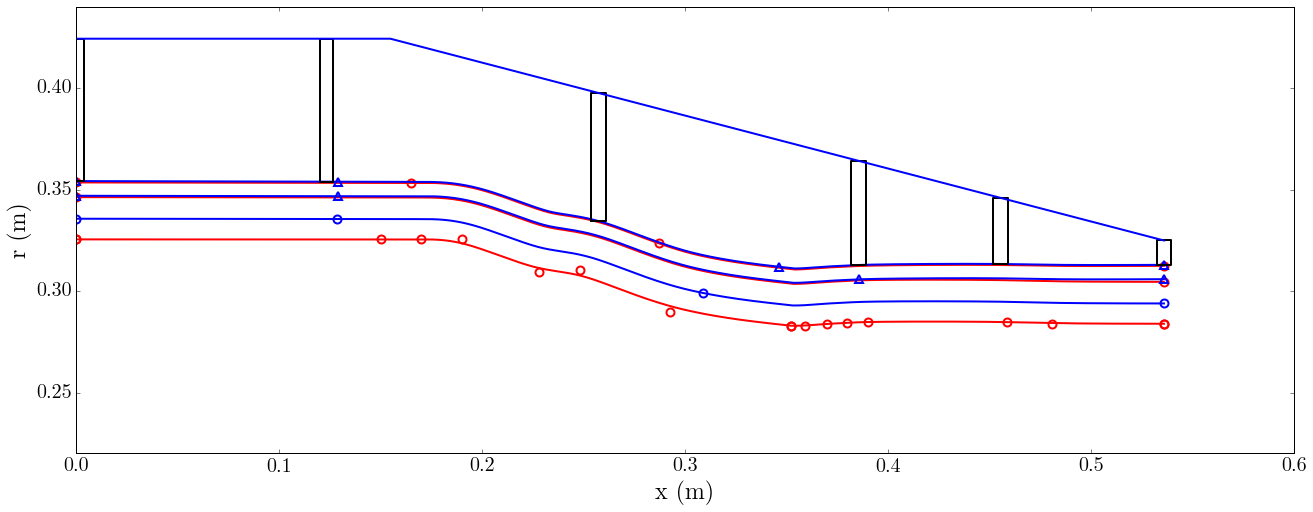
\includegraphics[scale=0.35]{figs/det-lo-optimal-shape.png}
\end{center}
\end{figure}

\begin{table}
\caption[Equivalent low-fidelity deterministic optimization objective and constraint values]{Value of objective function and constraints at equivalent low-fidelity deterministic optimum.}
\label{tab:det-lo-optimal-values}
\begin{center}
\begin{tabular}[]{ c | c | c | c }
\textbf{Description} & \textbf{Notation} & \textbf{Initial Value} & \textbf{Optimal Value} \\ \hline
Mass & $M$ & 118.74 & 32.843833 \\ \hline
Thrust & $F$ & 21475.92 & 21500.000632 \\ \hline
Inner load layer P-norm of temperature ratio & $g_1(\sfrac{T_2}{T_{max,2}})$ & 0.680 & 0.437059 \\ \hline
Thermal layer P-norm of failure criterion & $g_2(S_1(\sigma_1))$ & 0.112 & 0.122024 \\ \hline
Inner load layer P-norm of failure criterion & $g_3(S_2(\sigma_2))$ & 0.034 & 0.050842 \\ \hline
Middle load layer P-norm of failure criterion & $g_4(S_3(\sigma_3))$ & 0.210 & 0.212316 \\ \hline
Outer load layer P-norm of failure criterion & $g_5(S_4(\sigma_4))$ & 0.034 & 0.035907 \\ \hline
Stringers P-norm of failure criterion & $g_6(S_5(\sigma_5))$ & 0.035 & 0.024764 \\ \hline
Baffle 1 P-norm of failure criterion & $g_7(S_6(\sigma_6))$ & 0.012 & 0.002868 \\ \hline
Baffle 2 P-norm of failure criterion & $g_8(S_7(\sigma_7))$ & 0.009 & 0.007546 \\ \hline
Baffle 3 P-norm of failure criterion & $g_9(S_8(\sigma_8))$ & 0.010 & 0.006873 \\ \hline
Baffle 4 P-norm of failure criterion & $g_{10}(S_9(\sigma_9))$ & 0.006 & 0.004623 \\ \hline
Baffle 5 P-norm of failure criterion & $g_{11}(S_{10}(\sigma_{10}))$ & 0.007 & 0.002679 \\ \hline
Baffle 6 P-norm of failure criterion & $g_{12}(S_{11}(\sigma_{11}))$ & 0.006 & 0.002224 \\ \hline
\end{tabular}
\end{center}
\end{table}

\subsubsection{Discussion of Optimum}

The optimal nozzle shape shows a careful balance between the mass of the nozzle baffles and stringers and the mass of the nozzle wall, while at the same time finding a shape that generates enough thrust.

The overall wall shape is a nozzle that converges to the throat and remains flat until the exit. A flat post-throat shapes gives a lower nozzle wall mass compared to a diverging post-throat shape and is found here because the low-fidelity fluid analysis does not account for the detrimental shock/expansion phenomena that would occur with such a shape. The nozzle converges gradually to the throat due to a careful balance between baffle and wall mass (a steeper convergence would lead to a larger baffle). In fact, note that the converging portion of the nozzle wall is approximately parallel to the external aircraft shape. In addition, the nozzle wall has a small bump in the converging portion of the nozzle to decrease the baffle mass there.

As expected for a minimum mass problem, all wall layers, baffles, and stringers are as thin as possible. The exception is the air gap, which has the greatest possible thickness. It contributes to the nozzle mass indirectly since although the air is assumed to have no mass, the thickness of the air gap changes the radius of the upper wall layers and therefore their mass. Since the temperature constraint is not tight, it seems that a large air gap helps decrease the baffle mass more than the mass of the load layer increases. Lastly, the last three baffles have also been pushed as far right as possible to minimize their mass.

Although this is the critical loading condition, with the given material properties and minimum thicknesses, stresses and temperatures are not critical. Thinner wall layers would lead to higher temperatures and stresses. It appears that the middle titanium-honeycomb load layer is the most critical for stress.

\subsection{Medium-Fidelity Deterministic Optimization}

The optimization is run in parallel using 16 cores and terminates with the message \texttt{Current point cannot be improved upon} after 13 days and 10 major iterations. There are 4,599 total function evaluations including finite differences and no duplicate evaluations. This termination message is indicative of poor gradient accuracy, however after restarting the optimization at the solution found by NPSOL using a rescaled problem and the SNOPT optimization algorithm, it was found that the scaled optimization problem satisfies the specified optimality and constraint tolerances. As a result the constraint tolerance was tightened to $10^{-4}$ and SNOPT is currently being used to improve the design. However, in this document the NPSOL solution is presented.

\subsubsection{Optimum}

The optimal shape is shown in figure \ref{fig:det-med-optimal-shape}. Table \ref{tab:det-med-optimal-values} gives the values of the objective function and nonlinear constraints at the optimum. At the optimum 32 variable bounds are tight, 11 linear constraints are tight and the nonlinear thrust constraint is infeasible but within 0.197\% of its bound. The following observations are made about the solution:

\begin{enumerate}
\item The nozzle is as short as possible.
\item The throat is pushed as far to the right as possible.
\item The thermal layer, all load layers, stringers, and baffles are all as thin as possible.
\item B-spline coefficients have tended to cluster after the throat as they are pushed to the right (3 tight relative x-position constraints).
\item A flat diverging section is apparent. The B-spline coefficients to the immediate left and right of the throat are as low as possible, and there are 3 tight minimum slope constraints in the post-throat region.
\item Baffles 3 and 4 are as far apart as possible (notably in the converging section where the gap between the nozzle wall and exterior is greatest).
\item Baffles 4, 5, and 6 are as close as possible.
\item The only active non-linear constraint is the thrust constraint which is infeasible with a value of 21,547.51 N.
\end{enumerate}

\begin{figure}
\caption{Optimal shape for equivalent medium-fidelity deterministic optimization for reliable DUU problem in equation \ref{eq:specific_reliable_equiv_deterministic_optim}.}
\label{fig:det-med-optimal-shape}
\begin{center}
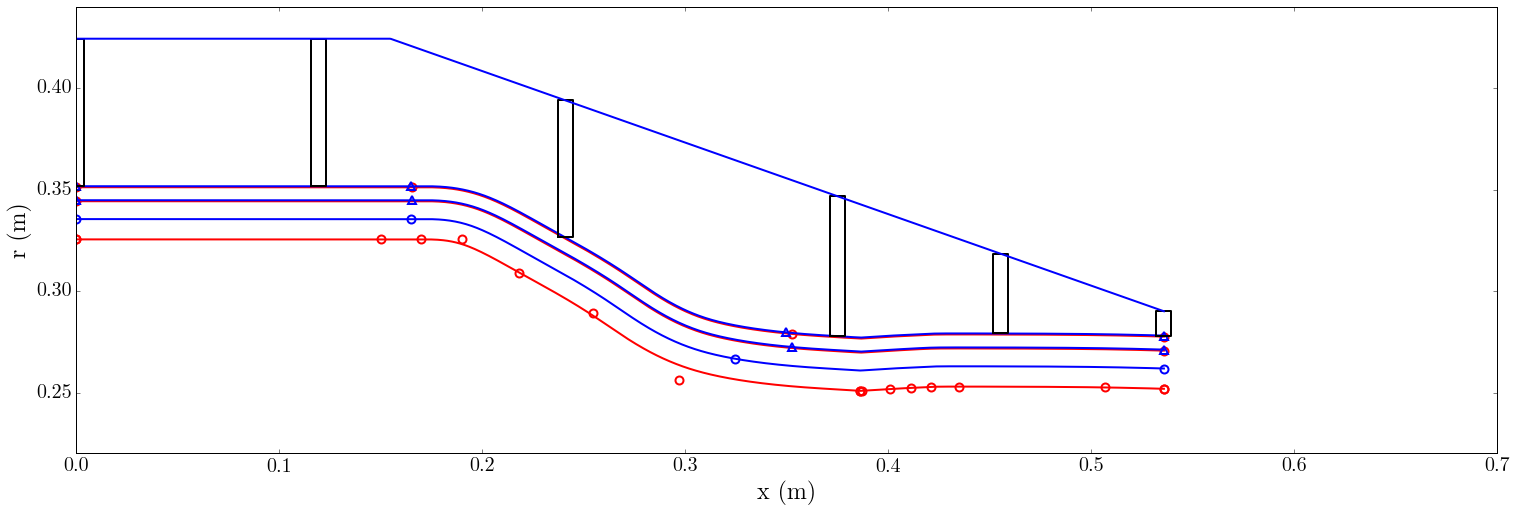
\includegraphics[scale=0.35]{figs/det-med-optimal-shape.png}
\end{center}
\end{figure}


\begin{table}
\caption[Equivalent medium-fidelity deterministic optimization objective and constraint values]{Value of objective function and constraints at equivalent medium-fidelity deterministic optimum.}
\label{tab:det-med-optimal-values}
\begin{center}
\begin{tabular}[]{ c | c | c | c }
\textbf{Description} & \textbf{Notation} & \textbf{Initial Value} & \textbf{Optimal Value} \\ \hline
Mass & $M$ & 156.34  & 31.860419 \\ \hline
Thrust & $F$ & 24064.73 & 21457.512003 \\ \hline
Inner load layer P-norm of temperature ratio & $g_1(\sfrac{T_2}{T_{max,2}})$ & 0.380 & 0.457780 \\ \hline
Thermal layer P-norm of failure criterion & $g_2(S_1(\sigma_1))$ & 0.108 & 0.115759 \\ \hline
Inner load layer P-norm of failure criterion & $g_3(S_2(\sigma_2))$ & 0.022 & 0.057282 \\ \hline
Middle load layer P-norm of failure criterion & $g_4(S_3(\sigma_3))$ & 0.002 & 0.001445 \\ \hline
Outer load layer P-norm of failure criterion & $g_5(S_4(\sigma_4))$ & 0.044 & 0.050168 \\ \hline
Stringers P-norm of failure criterion & $g_6(S_5(\sigma_5))$ & 0.044 & 0.025821 \\ \hline
Baffle 1 P-norm of failure criterion & $g_7(S_6(\sigma_6))$ & 0.003 & 0.002771 \\ \hline
Baffle 2 P-norm of failure criterion & $g_8(S_7(\sigma_7))$ & 0.007 & 0.004510 \\ \hline
Baffle 3 P-norm of failure criterion & $g_9(S_8(\sigma_8))$ & 0.005 & 0.004155 \\ \hline
Baffle 4 P-norm of failure criterion & $g_{10}(S_9(\sigma_9))$ & 0.009 & 0.001439 \\ \hline
Baffle 5 P-norm of failure criterion & $g_{11}(S_{10}(\sigma_{10}))$ & 0.012 & 0.001854 \\ \hline
Baffle 6 P-norm of failure criterion & $g_{12}(S_{11}(\sigma_{11}))$ & 0.007 & 0.001135 \\ \hline
\end{tabular}
\end{center}
\end{table}

\subsubsection{Discussion of Optimum}

The optimal nozzle shape again shows a careful balance between the mass allocated to the baffles and the shape of the inner wall. Clearly wall layers of minimum thickness are beneficial. The thrust constraint is clearly the most critical, followed by the temperature constraint for the inner load layer. The most critical stress constraints are the thermal layer and the Gr-BMI layers in the load layer. Note here that the air gap is not maximized.

The overall wall shape is a nozzle that converges smoothly to the throat and remains flat until the exit. Baffles have been positioned around this geometry so as to have the least mass, namely in the spaces where the nozzle wall is closest to the nozzle exterior. As a result, the optimal nozzle configuration is likely highly dependent on the exterior geometry.

\subsubsection{Comparison of Low- and Medium-Fidelity Optimums}

Interestingly the low- and medium-fidelity optimal geometries share many common features such as a flat diverging section, minimum wall layer thicknesses, and baffle placement sensitive to the exterior geometry and inner wall shape. Similar trends in stresses are observed.

Several notable differences exist. First, the air gap is maximized in the low-fidelity optimization where as it is not in the medium-fidelity optimization, thus leading to a higher temperature in the inner load layer. Next, although both nozzle shapes have a smooth divergent section, the medium-fidelity shape is smoother without the bump found in the low-fidelity shape. Next, the medium-fidelity nozzle analysis generates a higher thrust than that predicted by the low-fidelity nozzle analysis. As a result, the medium-fidelity nozzle can have a smaller throat and thereby lower mass.

\section{\texttt{MULTI-F} Verification} \label{sec:verification}

Verification of the code installation can be done by comparing the code's output for two fidelity levels using an example config file. The expected output is provided on the Github wiki.

\section{Appendix} \label{sec:appendix}

\subsection{Wall Parameterization}

Figures \ref{fig:wall_param_bspline} and \ref{fig:wall_param_layer} give a schematic of the degrees of freedom for two choices of parameterization, the 21-dof B-spline inner wall, and the 6-dof layer thickness. Figure \ref{fig:throatDofs} shows careful management of degrees of freedom near the throat in order to avoid issues during optimization.

\begin{figure}
\caption{21-dof B-spline parameterization for axisymmetric shape of inner wall.}
\label{fig:wall_param_bspline}
\begin{center}
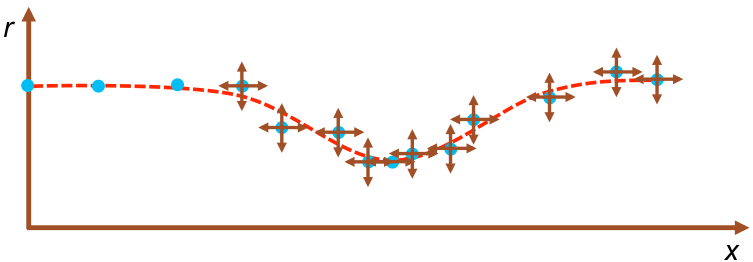
\includegraphics[scale=0.4]{figs/bspline_parameterization.png}
\end{center}
\end{figure}

\begin{figure}
\caption{Schematic of control points governing the nozzle throat and corresponding degrees of freedom. The black line denotes the B-spline shape of the nozzle inner wall, control points are denoted by red circles, and degrees of freedom are denoted by blue arrows. The boxed region indicates the throat of the nozzle. Note that there are 3 control points that govern the shape of the nozzle throat, and only 3 degrees of freedom. That is to say, the y-coordinate of all 3 control points is governed by one variable and the x-coordinates of all 3 control points are governed by two variables (in fact, the first two control points are duplicated). This gives much better control over the location of the throat.}
\label{fig:throatDofs}
\begin{center}
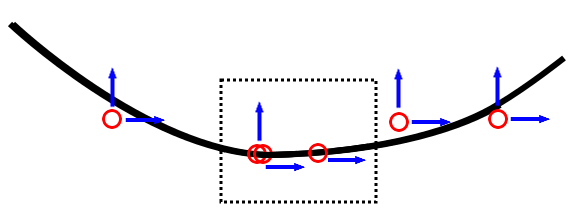
\includegraphics[scale=0.5]{figs/throat_area_control_points.png}
\end{center}
\end{figure}

\begin{figure}
\caption{6-dof piecewise-linear parameterization for axisymmetric wall layer thickness.}
\label{fig:wall_param_layer}
\begin{center}
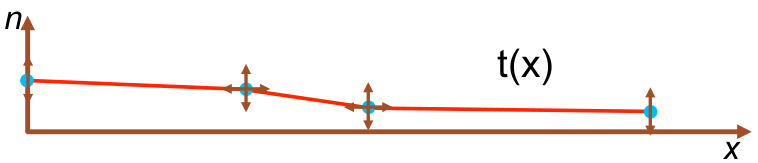
\includegraphics[scale=0.4]{figs/piecewiselinear_parameterization.png}
\end{center}
\end{figure}

\subsection{Basis-splines}

The inner wall of the nozzle is parameterized using a 3rd degree basis spline (B-spline). Although determination of a B-spline's shape requires the numerical solution of a recursive algorithm, B-splines have several nice properties including 1) they are a generalization of all splines, 2) in general, overfitting is avoided, and 3) any segment lies in the convex hull of neighboring control points \cite{prautzsch_bezier_2002}. Equation~\ref{eq:Bspline} defines the B-spline $s(t)$:

\begin{equation}
\label{eq:Bspline}
s(t) = \sum_i^N c_i N_i^n(t)
\end{equation}

where there are $N$ control points $c_i$ and $N$ basis functions $N_i$ of order $n$. The basis functions depend on the additional definition of a knots vector and can be determined using de Boor's algorithm \cite{prautzsch_bezier_2002}. In this work, the knots vector is assumed to be fixed and equally spaced.

For this problem, the nozzle's shape is changed by altering the coefficients $c_i$ of the B-spline, although one could also change the knots as well. Each coefficient has two degrees of freedom in the $\hat{x}$ and $\hat{r}$ directions, however not all degrees of freedom are unrestrained. For example, the inlet diameter and horizontal portion of the nozzle inlet is taken to be fixed. In addition, degrees of freedom are removed from B-spline coefficients near the nozzle throat so that only one coefficient's degree of freedom changes the radius of the throat.

\subsection{Kresselmeier-Steinhauser Function}

The Kresselmeier-Steinhauser function (KS-function) is a constraint agglomeration function of the form:

\begin{equation}
\label{eq:ks_function}
g(z) = \frac{1}{p} \textrm{log} \left( \sum_i^N e^{pz_i} \right)
\end{equation}

where $p$ is a constant usually chosen to be around 50, $z$ is vector of $N$ constraint values. For $\leq$ constraints, the KS-function overapproximates the constraints. As $p$ increases, the KS-function approaches the value $\textrm{max}(z)$. Based on preliminary analysis with different values of $p$ for the KS-function (30, 40, 50, and 60), it appears that the KS-function is too conservative, at least for normalized stress failure criteria and normalized temperatures used in constraints.

\subsection{Modified P-norm Function}

The modified P-norm function (PN-function) is a constraint agglomeration function of the form:

\begin{equation}
\label{eq:pn_function}
g(z) = \left( \frac{1}{N} \sum_i^N z_i^p \right)^{\frac{1}{p}}
\end{equation}

where $p$ is a constant usually chosen to be around 8 and $z$ is a vector of $N$ constraint values. For $\leq$ constaints, the modified P-norm function underapproximates the constraints. As $p$ increases, the PN-function approaches the value $\textrm{max}(z)$, however numerical difficulties ensue with too large a value of $p$. For values of $z$ around 1, the P-norm function appears approach the value $\textrm{max}(z)$, thus for normalized stress failure criteria and normalized temperatures used in constraints it appears to be a good option.



\bibliography{nozzle-optimization-problem-bibliography}
\bibliographystyle{aiaa}

\end{document}

%%% Local Variables:
%%% mode: latex
%%% TeX-master: t
%%% End:

\begin{table}
\caption{CMC: Macroscopic laminate material properties for the heat layer's ceramic matrix composite (CMC). Properties are taken from [0,90]4s weave Nextel 312/Silicon oxycarbide ceramic composite experimental data after 500 hours of oxidation at $600^{\circ}$C \cite{bansal_handbook_2005}.}
\label{tab:matPropCMC_detailed}
\begin{center}
\begin{tabular}[]{ c | c | c | c }
\textbf{Property} & \textbf{Units} & \textbf{Nominal Value} & \textbf{Distribution} \\ \hline
$\rho$ & $\frac{\textrm{kg}}{\textrm{m}^3}$ & 2410 & $\textrm{ln}\mathcal{N}(7.7804,0.0028)$ \\ \hline
$E_{1} = E_{2}$ & GPa & 67.1 & $\mathcal{N}(67.1,3.7^2)$ \\ \hline
$G_{12}$ & GPa & unknown & \\ \hline
$\nu_{12} = \nu_{21}$ & unknown & & \\ \hline
$\mu_{1,12} = \mu_{2,12}$ & & 0.0 & \\ \hline
$\mu_{12,1} = \mu_{12,2}$ & & 0.0 & \\ \hline
$k_{1} = k_{2}$ & $\frac{\textrm{W}}{\textrm{m-K}}$ & 1.58 & $\mathcal{U}(\pm3\%)$ \\ \hline
$k_{3}$ & $\frac{\textrm{W}}{\textrm{m-K}}$ & 1.4 & $\mathcal{U}(\pm3\%)$ \\ \hline
%$k$* & $\frac{\textrm{W}}{\textrm{m-K}}$ & 1.4 & $\mathcal{U}(\pm3\%)$ \\ \hline
$\alpha_{1} = \alpha_{2}$ & $\textrm{K}^{-1} \times 10^{-6}$ & 0.24 & \\ \hline
$\alpha_{3}$ & $\textrm{K}^{-1} \times 10^{-6}$ & 0.17  & \\ \hline
$\alpha_{12}$ & $\textrm{K}^{-1} \times 10^{-6}$ & 0.0 & \\ \hline \hline
$T_{max}$ & K & 973 & \\ \hline
$\epsilon_{f,2} = \epsilon_{f,2}$ & \% & 0.07 & $\mathcal{N}(0.07,0.01^2)$ \\ \hline
$\sigma_{f,1} = \sigma_{f_2}$ tension (compression) & MPa & 49.2 (120) & $\mathcal{N}(49.2,2.0^2)$ ($\mathcal{N}(120,28^2)$)\\ \hline
$\sigma_{f,3}$ tension (compression) & MPa &  & \\ \hline
$\sigma_{f,12}$ (ultimate) & MPa & 14.3 & $\mathcal{N}(14.3,0.5^2)$ \\ \hline
\end{tabular} \\
%*$k_1 = k_2 = 1.58$, however $k_3 = 1.4$ and is the dominant \\direction along which heat is removed from the nozzle.
\end{center}
\end{table}

\begin{table}
\caption{GR-BMI: Macroscopic laminate material properties for the load layer's Graphite/Bismaleimide (GR-BMI) composite layers. The macroscopic properties are based on experimental data\cite{cycom_2011,hextow_2016} and classical laminate analysis\cite{nettles_basic_1994} for a [+45,0,-45,90]2s laminate with a 60\% fiber volume at $24^{\circ}$C.}
\label{tab:matPropGR-BMI_detailed}
\begin{center}
\begin{tabular}[]{ c | c | c | c }
\textbf{Property} & \textbf{Units} & \textbf{Nominal Value} & \textbf{Distribution} \\ \hline
$\rho$ & $\frac{\textrm{kg}}{\textrm{m}^3}$ & 1568 & \\ \hline
$E_{1} = E_{2}$ & GPa & 60 & $\mathcal{U}(57,63)$ \\ \hline
$G_{12}$ & GPa & 23.31 & \\ \hline
$\nu_{12} = \nu_{21}$ & & 0.344 & \\ \hline
$\mu_{1,12} = \mu_{2,12}$ & & 0.0 & \\ \hline
$\mu_{12,1} = \mu_{12,2}$ & & 0.0 & \\ \hline
$k_{1} = k_{2}$ & $\frac{\textrm{W}}{\textrm{m-K}}$ & 3.377 & \\ \hline
$k_{3}$ & $\frac{\textrm{W}}{\textrm{m-K}}$ & 3.414 & \\ \hline
$\alpha_{1} = \alpha_{2}$ & $\textrm{K}^{-1} \times 10^{-6}$ & 1.200 & \\ \hline
$\alpha_{12}$ & $\textrm{K}^{-1} \times 10^{-6}$ & 0.0 & \\ \hline \hline
$T_{max}$ & K & 505 & \\ \hline
$\sigma_{f,1} = \sigma_{f_2}$ tension (compression) & MPa & 448 (310) & \\ \hline
$\sigma_{f,3}$ tension (compression) & MPa & 103 (66) & \\ \hline
$\sigma_{f,12}$ & MPa & 103 & \\ \hline
\end{tabular}
\end{center}
\end{table}

%\begin{table}
%\caption{Relevant material properties for Graphite/Bismaleimide unidirectional composite (GR-BMI-UNI) used for stringers. The material properties are based on experimental data with a 60\% fiber volume at $24^{\circ}$C.}
%\label{tab:matPropGR-BMI-UNI_detailed}
%\begin{center}
%\begin{tabular}[]{ c | c | c | c }
%\textbf{Property} & \textbf{Units} & \textbf{Nominal Value} & \textbf{Distribution} \\ \hline
%Density & $\frac{\textrm{kg}}{\textrm{m}^3}$ & 1568 & \\ \hline
%$E_{1}$ & GPa & 160 & $\mathcal{U}(158,162)$ \\ \hline
%$E_{2}$ & GPa & 9.7 & \\ \hline
%$G_{12}$ & GPa & 5.9 & \\ \hline
%$\nu_{12} = \nu_{21}$ & & 0.7 & \\ \hline
%$\mu_{1,12} = \mu_{2,12}$ & & 0.0 & \\ \hline
%$\mu_{12,1} = \mu_{12,2}$ & & 0.0 & \\ \hline \hline
%$k_{1}$ & $\frac{\textrm{W}}{\textrm{m-K}}$ & 3.34 & \\ \hline
%$k_{2} = k_{3}$ & $\frac{\textrm{W}}{\textrm{m-K}}$ & 3.414 & \\ \hline
%$\alpha_{1}$ & $\textrm{K}^{-1} \times 10^{-6}$ & -1.62 & \\ \hline
%$\alpha_{2}$ & $\textrm{K}^{-1} \times 10^{-6}$ & 30.06 & \\ \hline
%$\alpha_{12}$ & $\textrm{K}^{-1} \times 10^{-6}$ & 0.0 & \\ \hline \hline
%$T_{max}$ & K & 505 & \\ \hline
%$\sigma_{f,1}$ tension (compression) & MPa & 2618 (1620) & \\ \hline
%$\sigma_{f,2}$ tension (compression) & MPa & 66 (66) & \\ \hline
%$\sigma_{f,3}$ tension (compression) & MPa & 66 (66) & \\ \hline
%$\sigma_{f,12}$ & MPa & 103 & \\ \hline
%\end{tabular}
%\end{center}
%\end{table}

\begin{table}
\caption{TI-HC: Macroscopic material properties for titanium honeycomb layer (TI-HC). Material properties are based on experimental data \cite{ko_thermal_1991} and Lewis and Nielson semi-theoretical model for thermal conductivity \cite{progelhof_methods_1976}.}
\label{tab:matPropTI-HC_detailed}
\begin{center}
\begin{tabular}[]{ c | c | c | c }
\textbf{Property} & \textbf{Units} & \textbf{Nominal Value} & \textbf{Distribution} \\ \hline
Volume fraction & & 0.02296 & N/A \\ \hline
$\rho$ & $\frac{\textrm{kg}}{\textrm{m}^3}$ & 101.696 & $\mathcal{U}(\pm1\textrm{\%})$ \\ \hline
$E_{1} = E_{2}$ & GPa & 0.1915 &  \\ \hline
$E_{3}$ & GPa & 1.915 & \\ \hline
$G_{12}$ & GPa & $4.2 \times 10^{-8}$ & \\ \hline
$G_{23}$ & GPa & 1.248 & \\ \hline
$G_{31}$ & GPa & 0.565 & \\ \hline
$\nu_{12}$ & & 0.00658 & \\ \hline
$\nu_{23} = \nu_{13}$ & & $0.643 \times 10^{-6}$ & \\ \hline
%$\mu_{1,12} = \mu_{2,12}$ & & 0.0 & \\ \hline
%$\mu_{12,1} = \mu_{12,2}$ & & 0.0 & \\ \hline
$k_{1} = k_{2}$ & $\frac{\textrm{W}}{\textrm{m-K}}$ & 0.153 & $\mathcal{U}(0.147,0.160)$ \\ \hline
$k_{3}$ & $\frac{\textrm{W}}{\textrm{m-K}}$ & 0.413 & $\mathcal{U}(0.403,0.421)$ \\ \hline
$\alpha_{1} = \alpha_{2}$ & $\textrm{K}^{-1} \times 10^{-6}$ & 0.18 & \\ \hline \hline
$T_{max}$ & K & 755 & \\ \hline
%$\sigma_{f,1} = \sigma_{f_2}$ tension (compression) & MPa &  & \\ \hline
$\sigma_{f,3}$ tension (compression) & MPa & 8.04 (2.11) & \\ \hline
%$\sigma_{f,12}$ & MPa & & \\ \hline
$\sigma_{f,31}$ & MPa & 2.16 & \\ \hline
$\sigma_{f,32}$ & MPa & 3.31 & \\ \hline
$\sigma_Y$ (pure Ti, grade 2) & MPa & 350.17 \\ \hline
\end{tabular}
\end{center}
\end{table}

%%% Local Variables:
%%% mode: latex
%%% TeX-master: t
%%% End:
